\documentclass[12pt,letterpaper]{article}

\usepackage{amsmath, amsthm}
\usepackage{microtype, parskip}
\usepackage[comma,numbers,sort&compress]{natbib}
\usepackage{lineno}
\usepackage{docmute}
\usepackage{caption, subcaption, multirow, morefloats, rotating}
\usepackage{wrapfig}

\frenchspacing

\begin{document}

\section*{Results}

\subsection*{Comparing the fits of the pure-presence and birth-death models}

% look at the posterior predictive checks
%   which model has better fit
%   what does that mean?
% need to inspect the posterior estimates in order to understand the differences
%   ecotype occurrence (pp), origination + survival (bd) probabilities
%   effect of mass on 
%     preservation (pp, bd)
%     occurrence (pp)
%     origination + survival (bd)
%   group-level covariates on 
%     occurrence (pp)
%     origination + survival (bd)


\begin{figure}[ht]
  \centering
  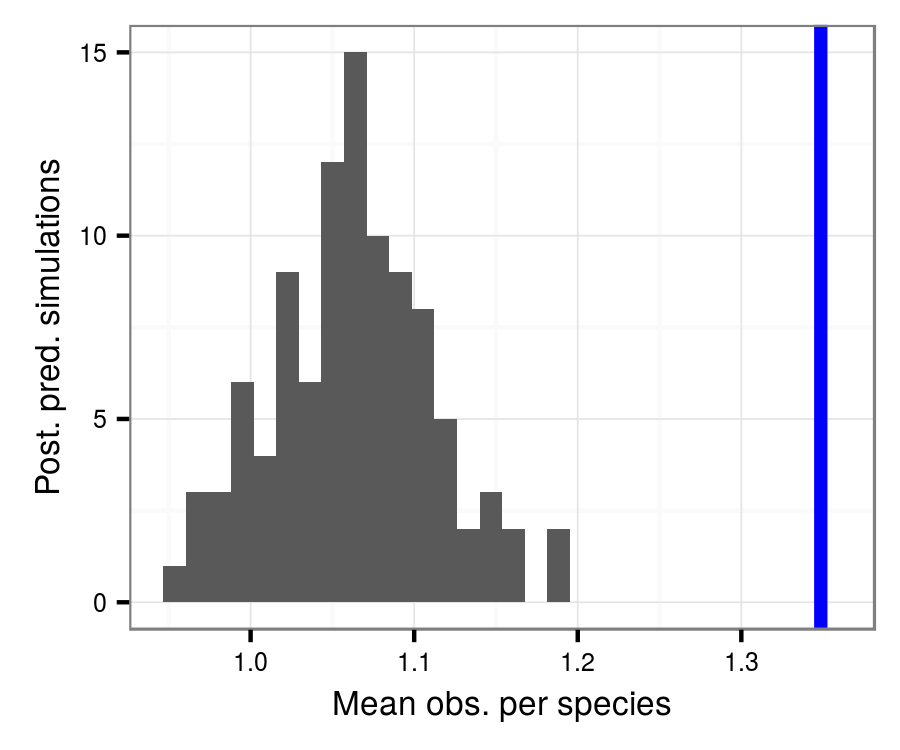
\includegraphics[width=\textwidth,height=0.4\textheight,keepaspectratio=true]{figure/pred_occ}
  \caption[Posterior predictive check for pure-presence model]{Comparison of the average observed number of occurrences per species (blue line) to the average number of occurrences from 100 posterior predictive datasets using the posterior estimates from the pure-presence model.}
  \label{fig:ppc_pure_presence}
\end{figure}

\begin{figure}[ht]
  \centering
  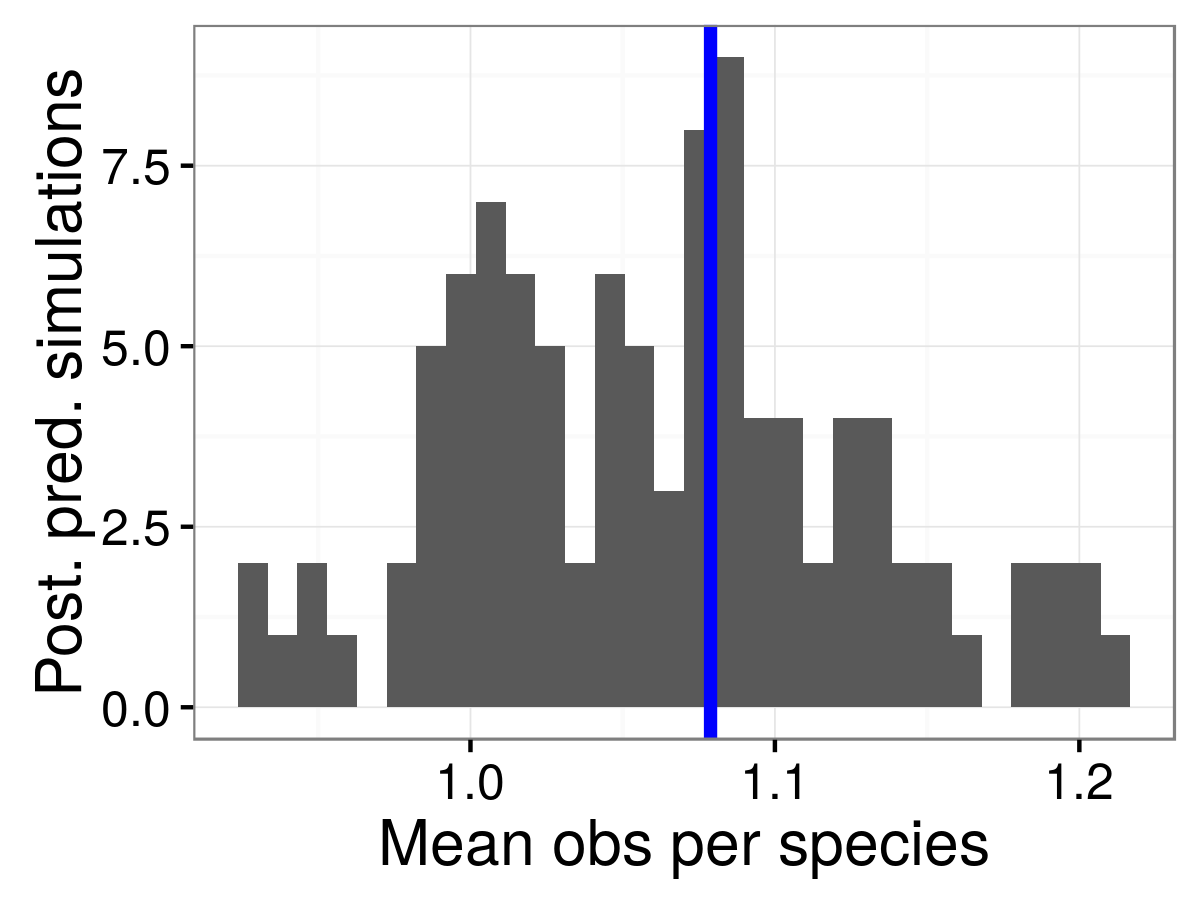
\includegraphics[width=\textwidth,height=0.4\textheight,keepaspectratio=true]{figure/pred_occ_bd}
  \caption[Posterior predictive check for birth-death model]{Comparison of the average observed number of occurrences per species (blue line) to the average number of occurrences from 100 posterior predictive datasets using the posterior estimate from the birth-death model.}
  \label{fig:ppc_birth_death}
\end{figure}

\begin{figure}[ht]
  \centering
  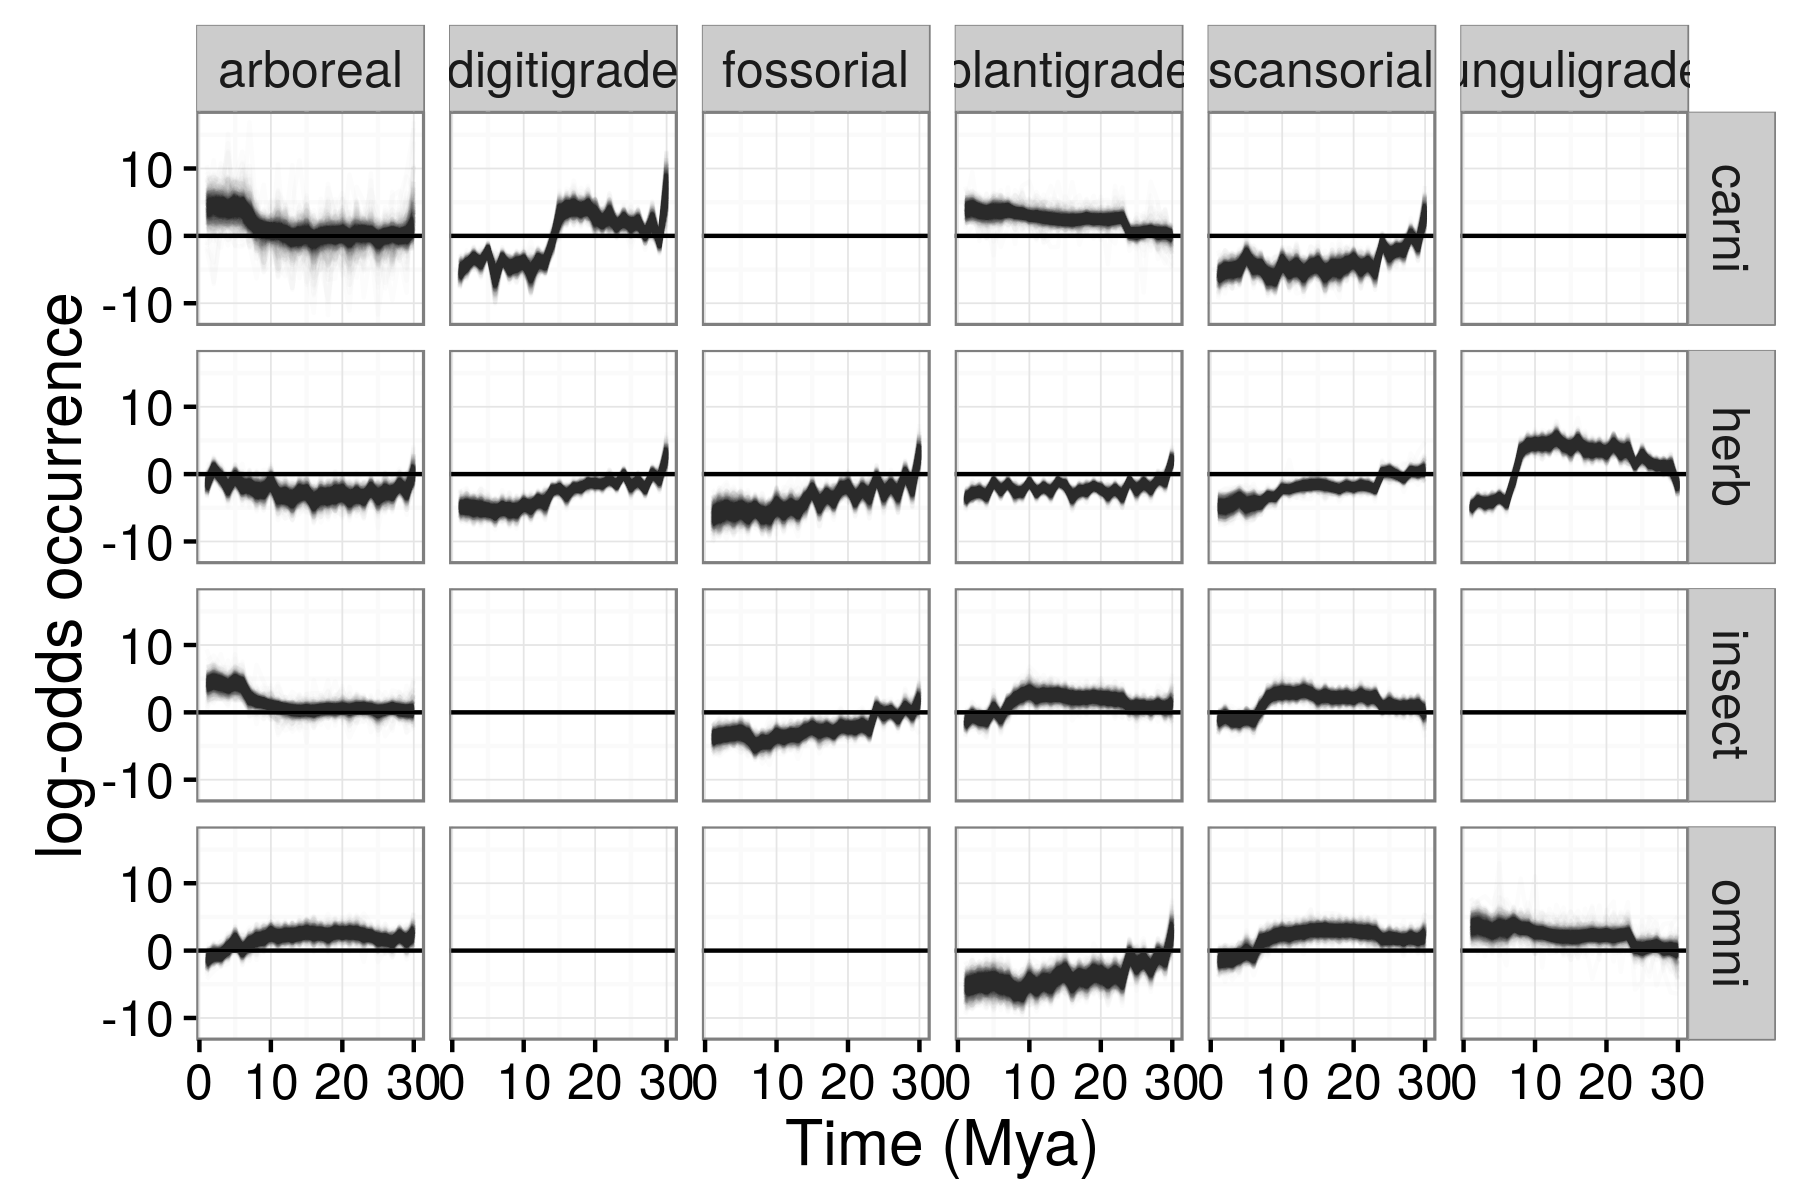
\includegraphics[width=\textwidth,height=0.8\textheight,keepaspectratio=true]{figure/ecotype_occurrence}
  \caption[Ecotype occurrence probability estimated from the pure-presence model]{Probability of a mammal ecotype occurring over time as estimated from the pure-presence model. Each panel depicts 100 random samples from the model's posterior. The columns are by locomotor category and rows by dietary category; their intersections are the observed and analyzed ecotypes. Panels with no lines are ecotypes not observed in the dataset.}
  \label{fig:eco_occur}
\end{figure}

\begin{figure}[ht]
  \centering
  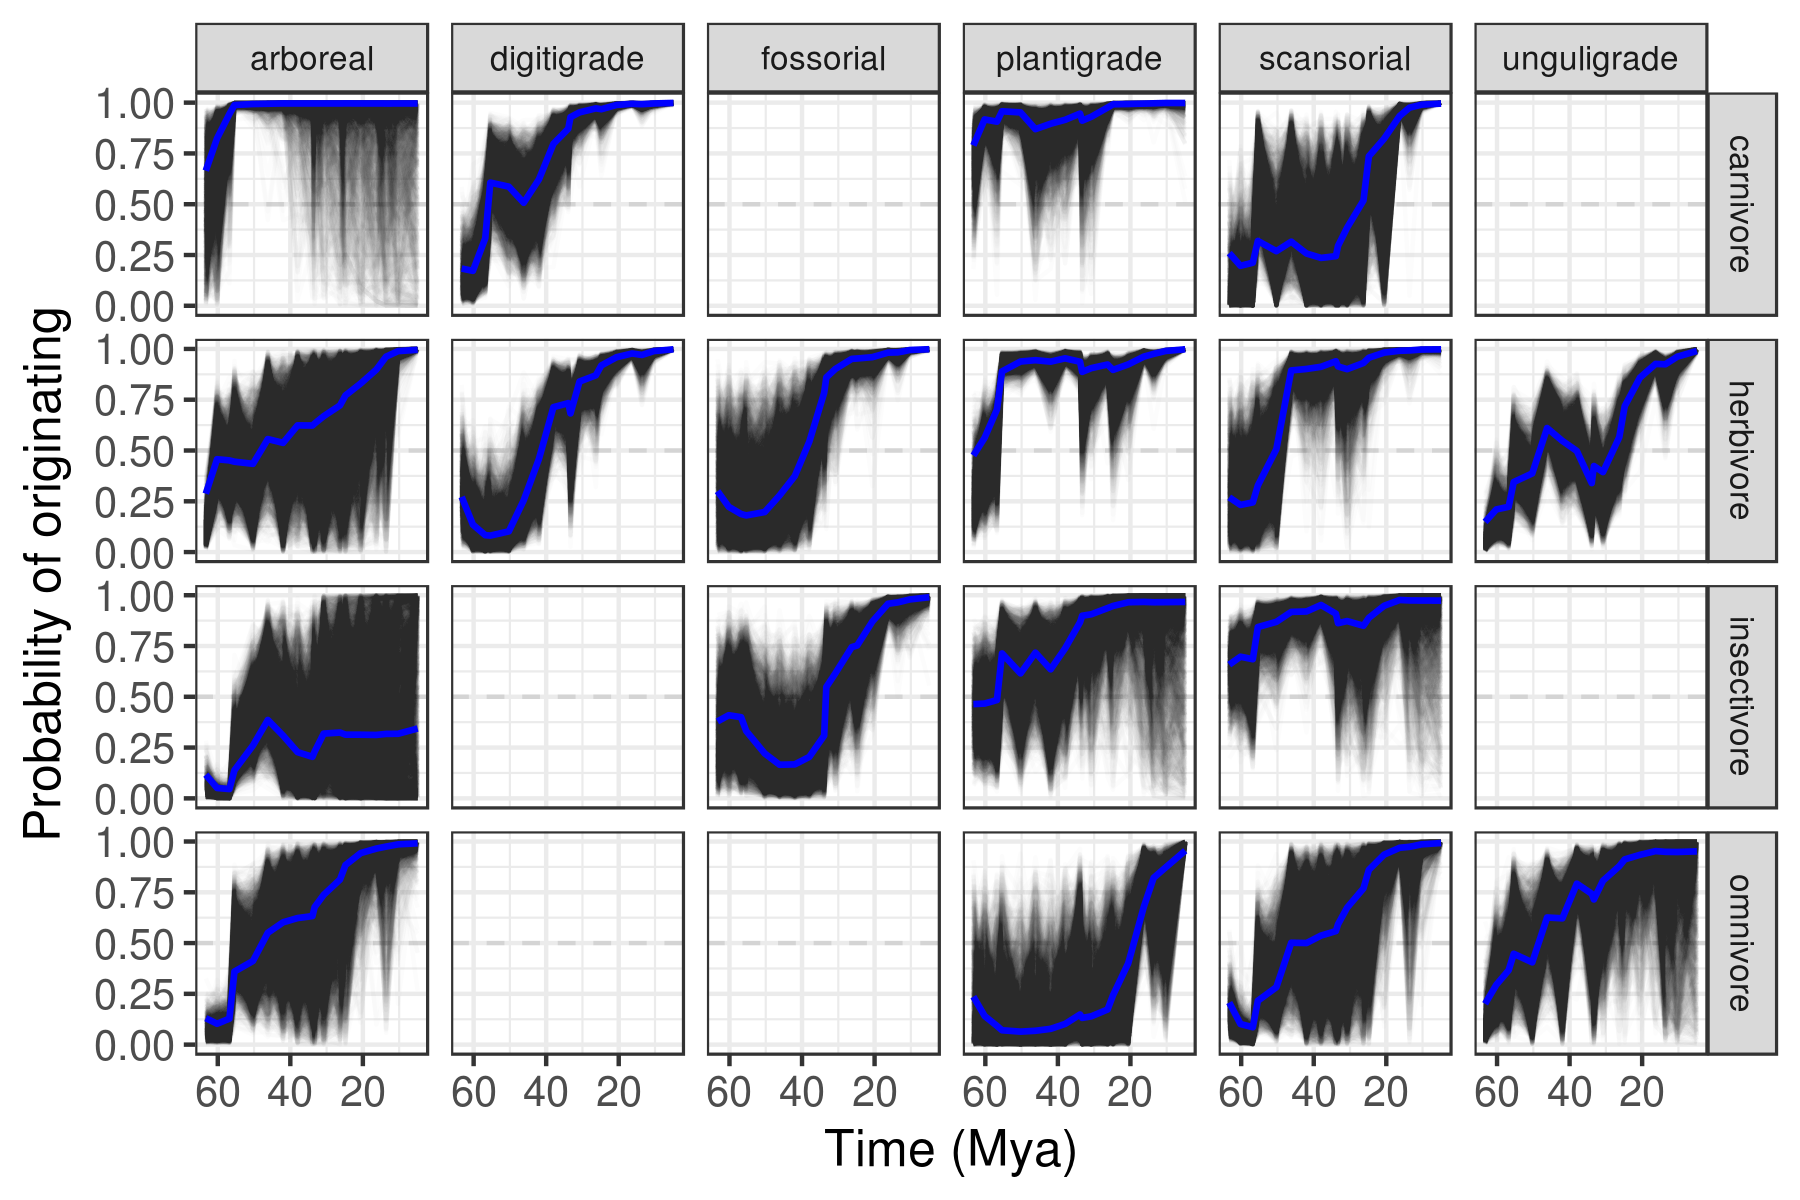
\includegraphics[width=\textwidth,height=0.8\textheight,keepaspectratio=true]{figure/ecotype_origin_bd}
  \caption[Ecotype origination probability estimated from the birth-death model]{Probability of a mammal ecotype origination probabliities at each time point as estimated from the birth-death model. Each panel depicts 100 random samples from the model's posterior. The columns are by locomotor category and rows by dietary category; their intersections are the observed and analyzed ecotypes. Panels with no lines are ecotypes not observed in the dataset.}
  \label{fig:eco_origin}
\end{figure}

\begin{figure}[ht]
  \centering
  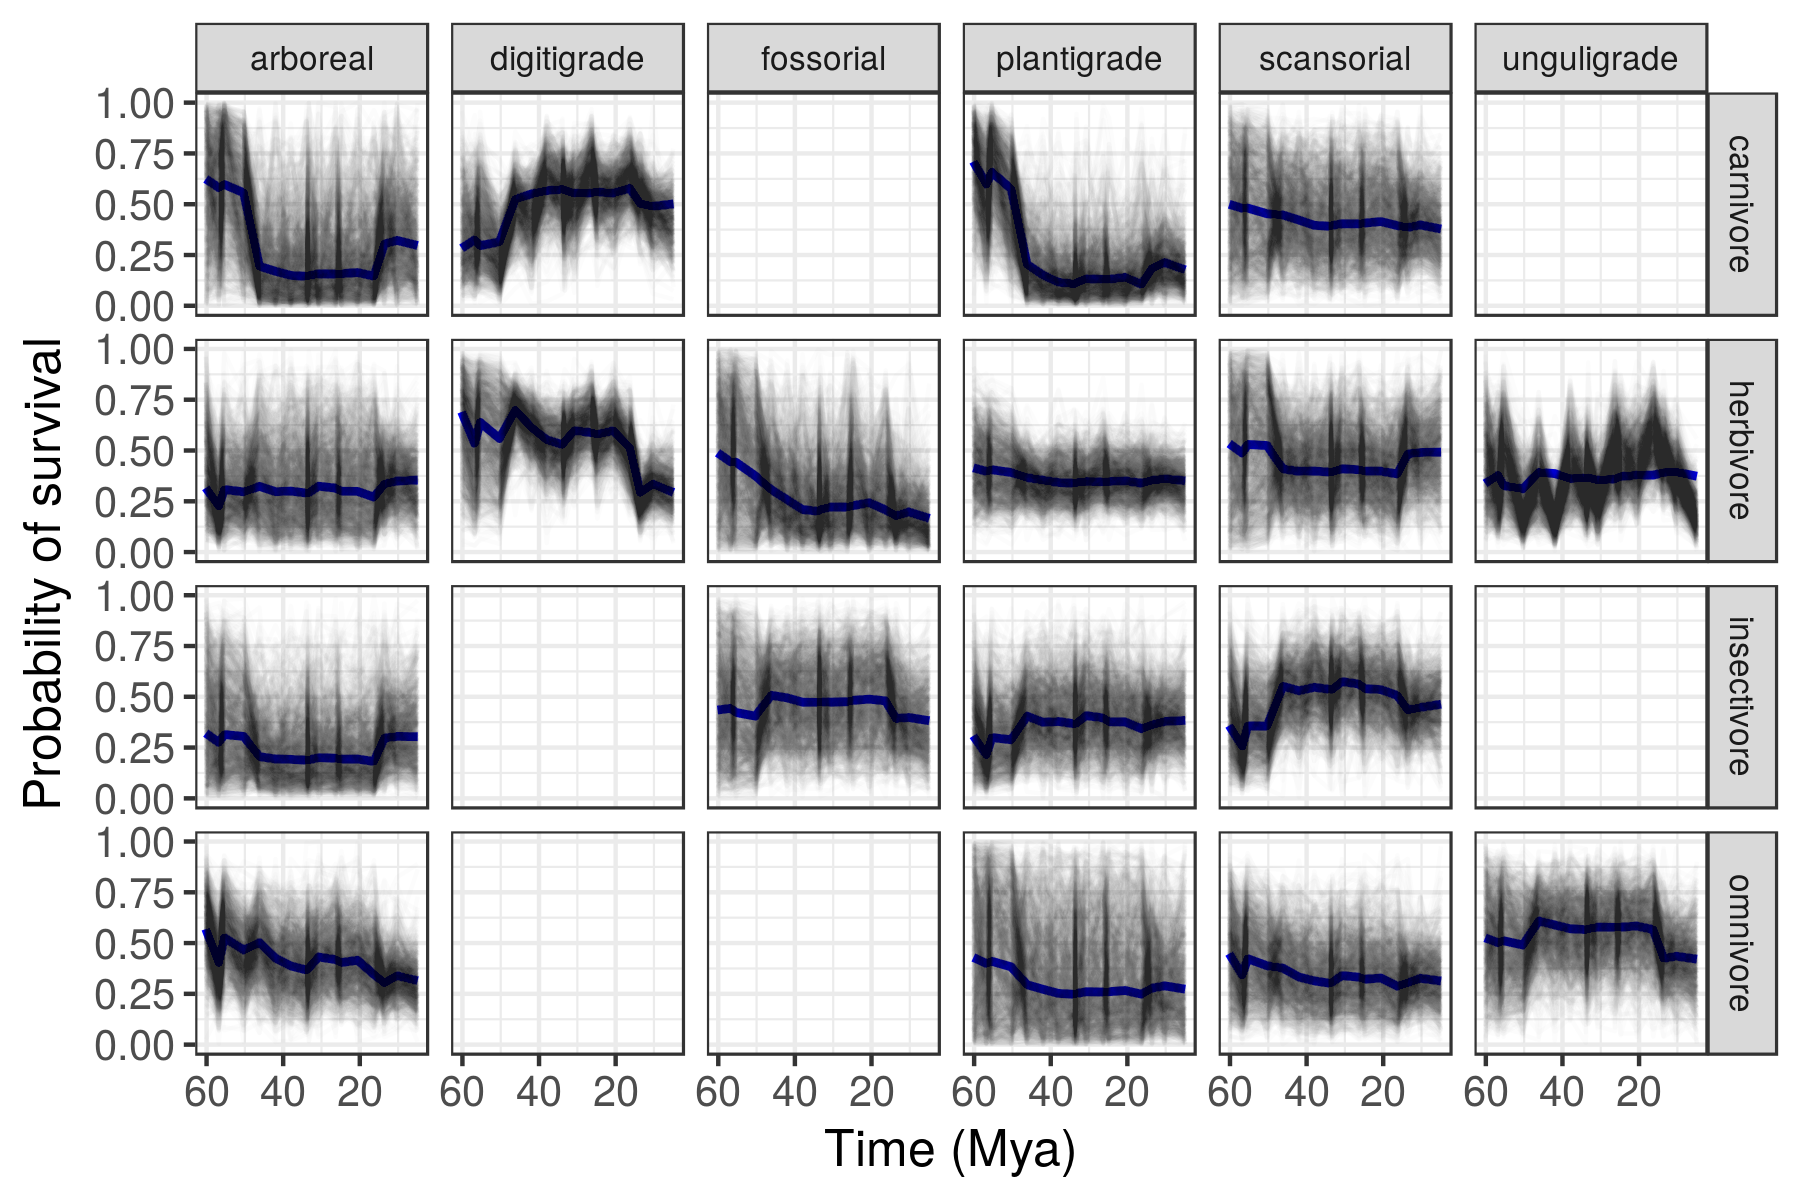
\includegraphics[width=\textwidth,height=0.8\textheight,keepaspectratio=true]{figure/ecotype_survival_bd}
  \caption[Ecotype survival probability estimated from the birth-death model]{Probability of a mammal ecotype survival probabilities at each time point as estimated from the birth-death model. Each panel depicts 100 random samples from the model's posterior. The columns are by locomotor category and rows by dietary category; their intersections are the observed and analyzed ecotypes. Panels with no lines are ecotypes not observed in the dataset.}
  \label{fig:eco_survival}
\end{figure}

\begin{figure}[ht]
  \centering
  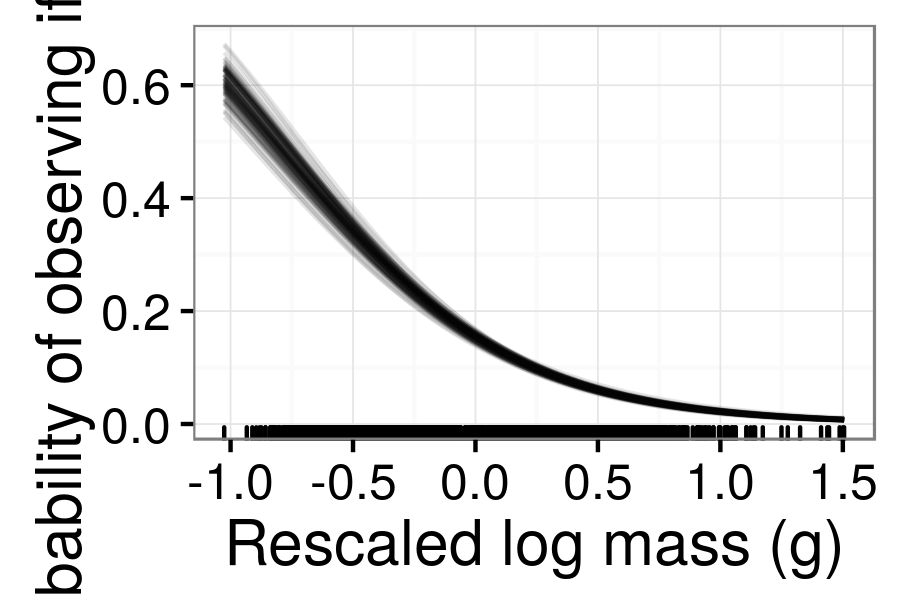
\includegraphics[width=\textwidth,height=0.8\textheight,keepaspectratio=true]{figure/mass_on_samp}
  \caption[Estimates of the effect of mass on observation probability from the pure-presence model]{Estimates of the effect of species mass on probability of observing a present species (\(p\)). Mass has been log-transformed, centered, and rescaled; this means that a mass of 0 corresponds to the mean of log-mass of all observed species and that mass is in standard deviation units. Estimates are from the pure-presence model.}
  \label{fig:mass_preserve_pure_pres}
\end{figure}

\begin{figure}[ht]
  \centering
  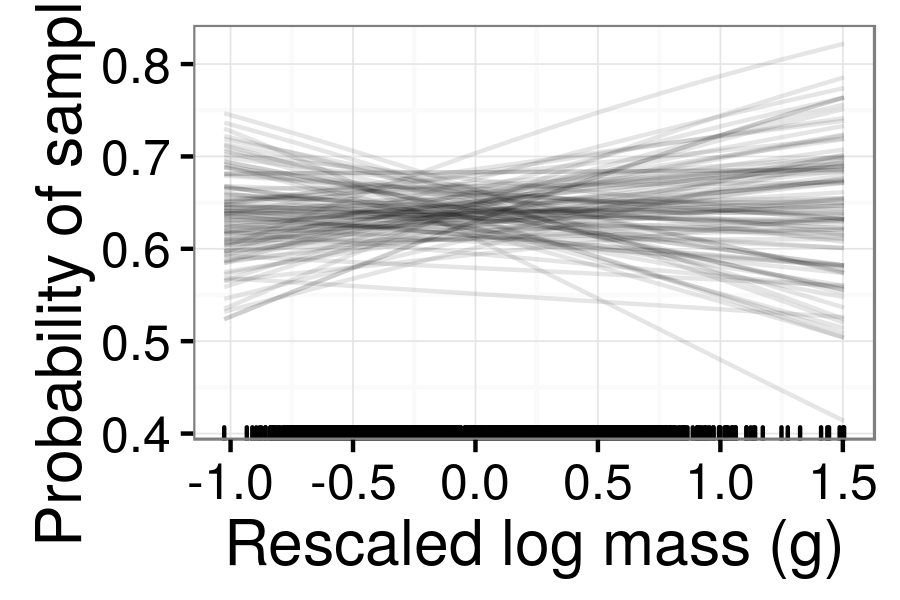
\includegraphics[width=\textwidth,height=0.8\textheight,keepaspectratio=true]{figure/mass_on_samp_bd}
  \caption[Estimates of the effect of mass on observation probability from the birth-death model]{Estimates of the effect of species mass on probability of observing a present species (\(p\)). Mass has been log-transformed, centered, and rescaled; this means that a mass of 0 corresponds to the mean of log-mass of all observed species and that mass is in standard deviation units. Estimates are from the birth-death model.}
  \label{fig:mass_preserve_bd}
\end{figure}

\begin{figure}[ht]
  \centering
  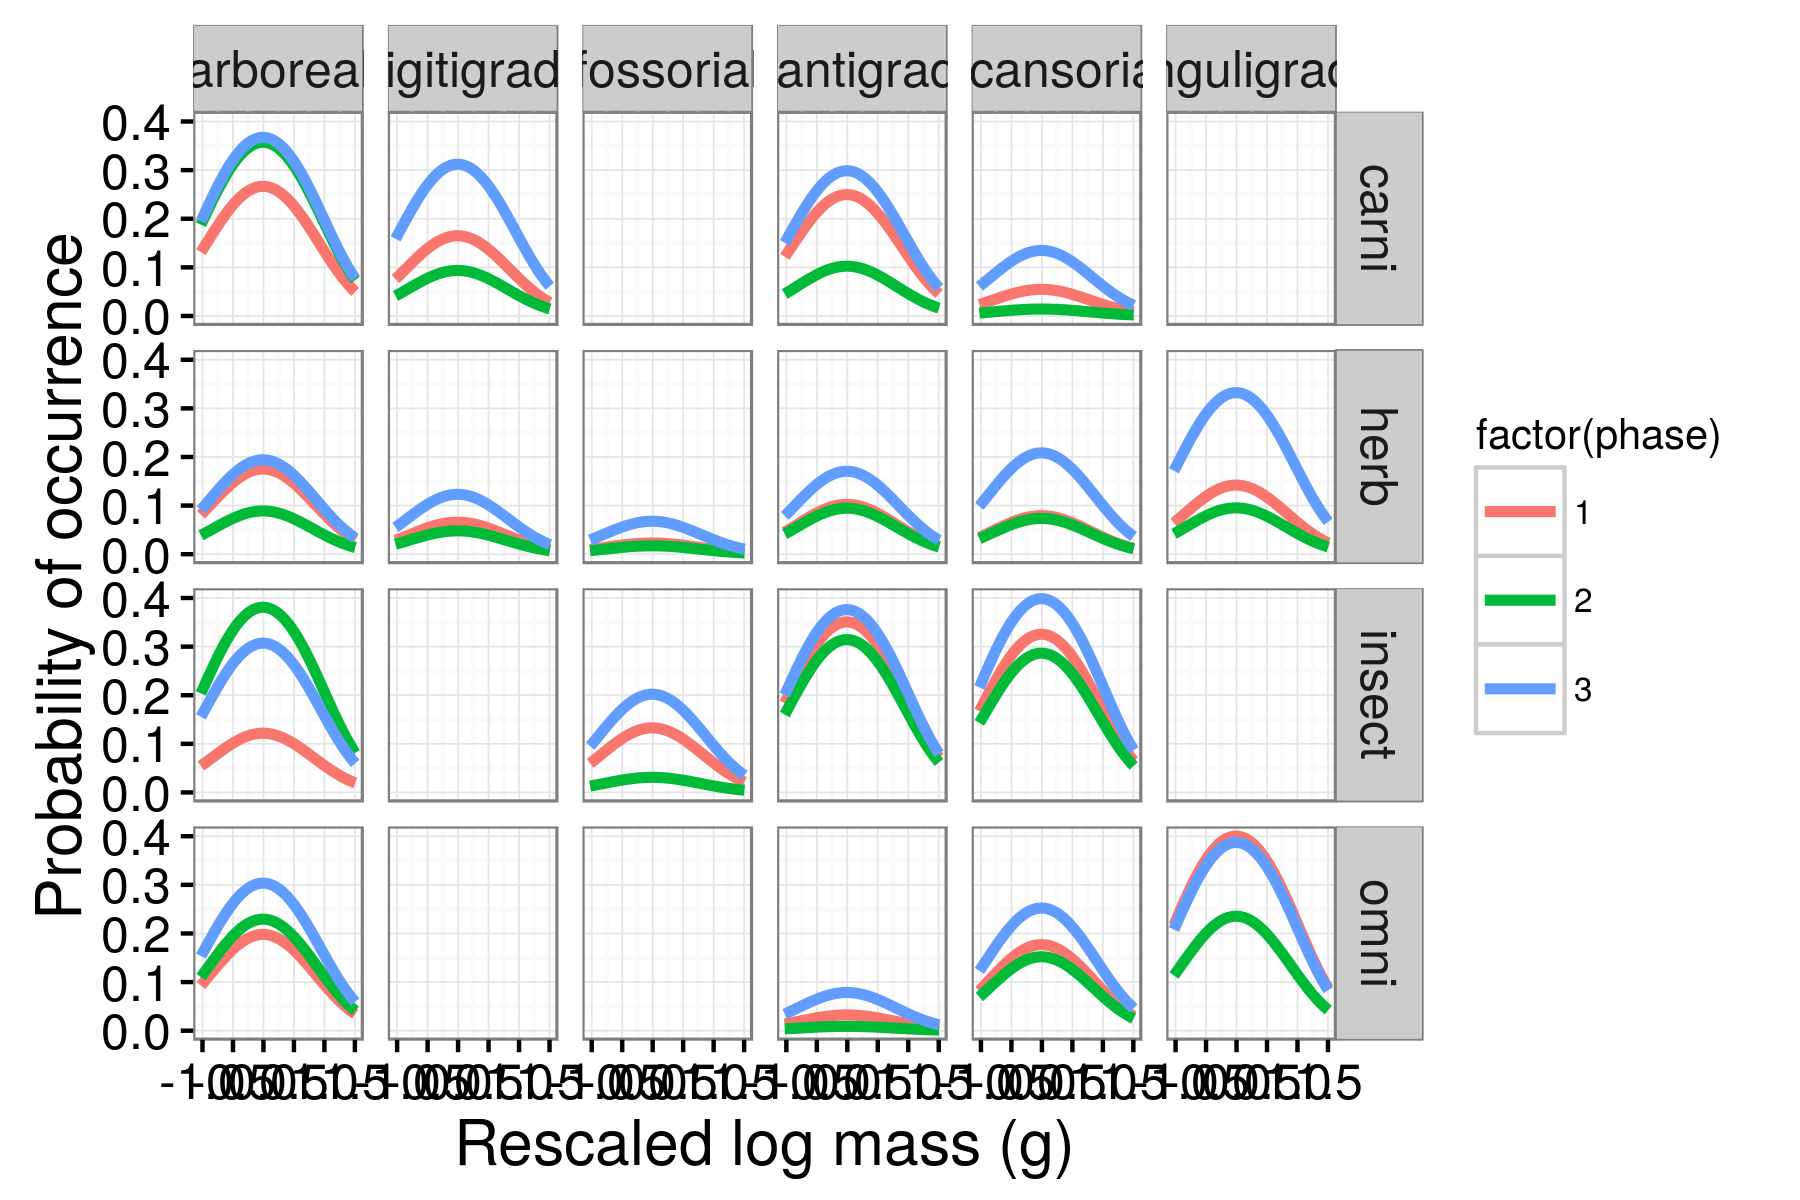
\includegraphics[width=\textwidth,height=0.8\textheight,keepaspectratio=true]{figure/mass_on_pres}
  \caption[Effect of mass on probability of species occurrence as estimated from the pure-presence model]{Mean estimate of the effect of species mass on the probability of a species occurrence for each of the three plant phases. The effect of mass is considered constant over time and that the only aspect of the model that changes with plant phase is the intercept of the relationship between mass and occurrence. The three plant phases are indicated by the color of the line. Mass has been log-transformed, centered, and rescaled; this means that a mass of 0 corresponds to the mean of log-mass of all observed species and that mass is in standard deviation units.}
  \label{fig:mass_occur}
\end{figure}

\begin{figure}[ht]
  \centering
  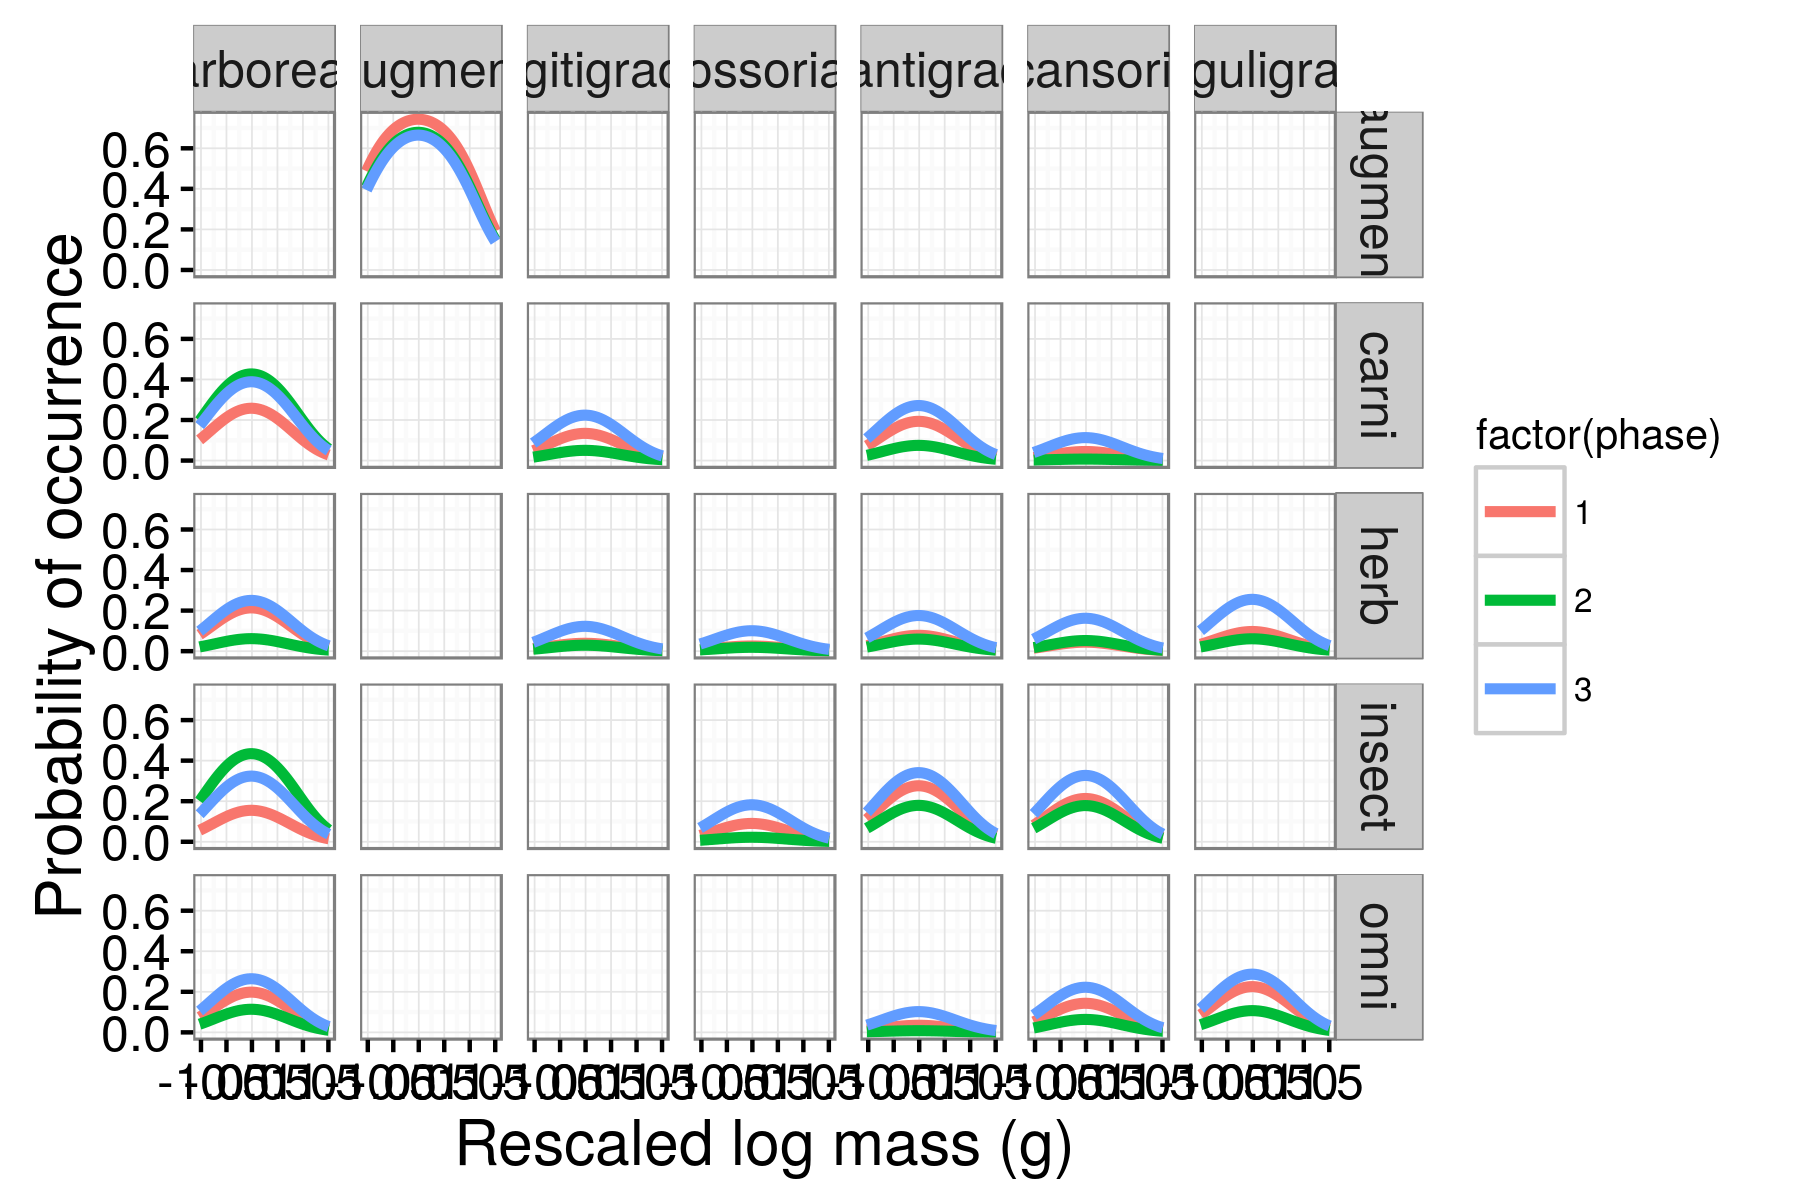
\includegraphics[width=\textwidth,height=0.8\textheight,keepaspectratio=true]{figure/mass_on_origin_bd}
  \caption[Effect of mass on probability of species origination as estimated from the birth-death model]{Mean estimate of the effect of species mass on the probability of a species originating for each of the three plant phases. The effect of mass is considered constant over time and that the only aspect of the model that changes with plant phase is the intercept of the relationship between mass and origination. The three plant phases are indicated by the color of the line. Mass has been log-transformed, centered, and rescaled; this means that a mass of 0 corresponds to the mean of log-mass of all observed species and that mass is in standard deviation units.}
  \label{fig:mass_origin}
\end{figure}

\begin{figure}[ht]
  \centering
  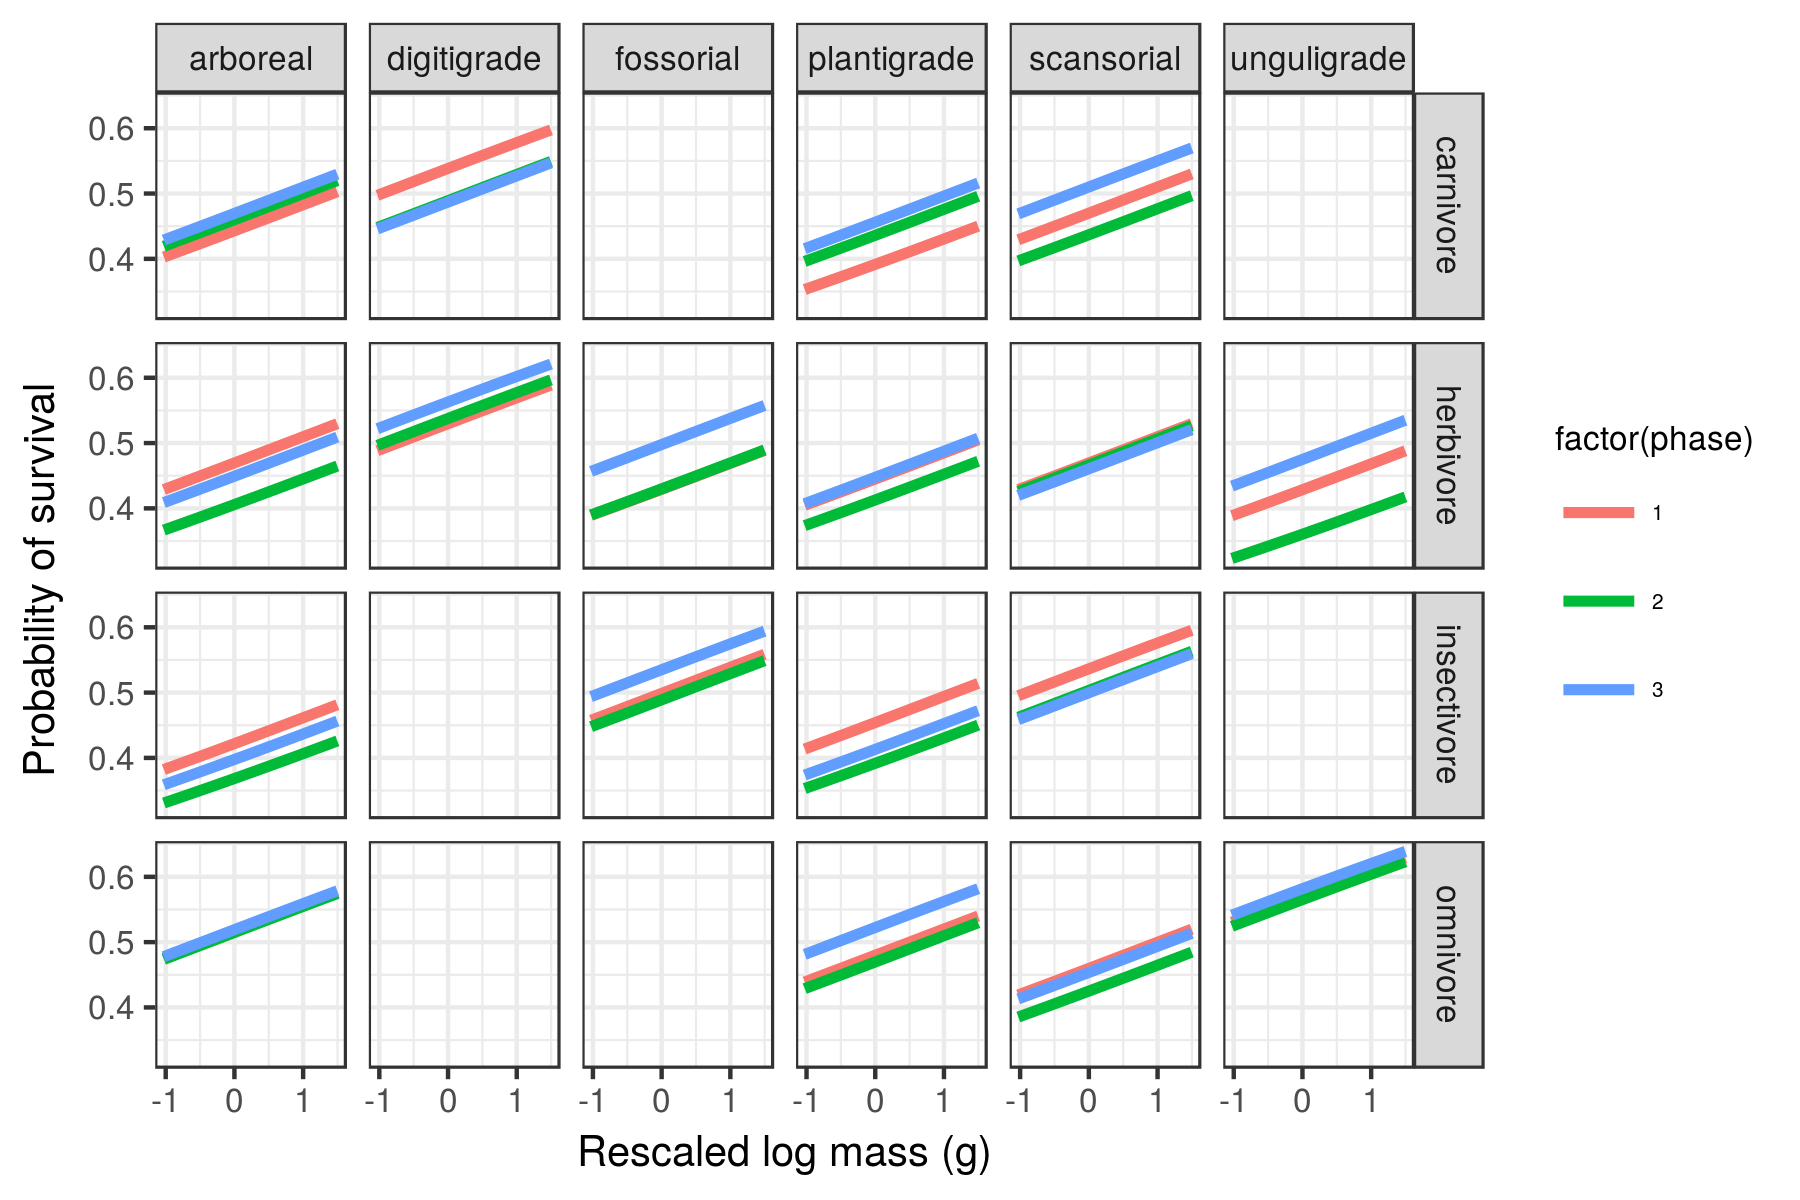
\includegraphics[width=\textwidth,height=0.8\textheight,keepaspectratio=true]{figure/mass_on_surv_bd}
  \caption[Effect of mass on probability of species survival as estimated from the birth-death model]{Mean estimate of the effect of species mass on the probability of a species survival for each of the three plant phases. The effect of mass is considered constant over time and that the only aspect of the model that changes with plant phase is the intercept of the relationship between mass and survival. The three plant phases are indicated by the color of the line. Mass has been log-transformed, centered, and rescaled; this means that a mass of 0 corresponds to the mean of log-mass of all observed species and that mass is in standard deviation units.}
  \label{fig:mass_survival}
\end{figure}

\begin{figure}[ht]
  \centering
  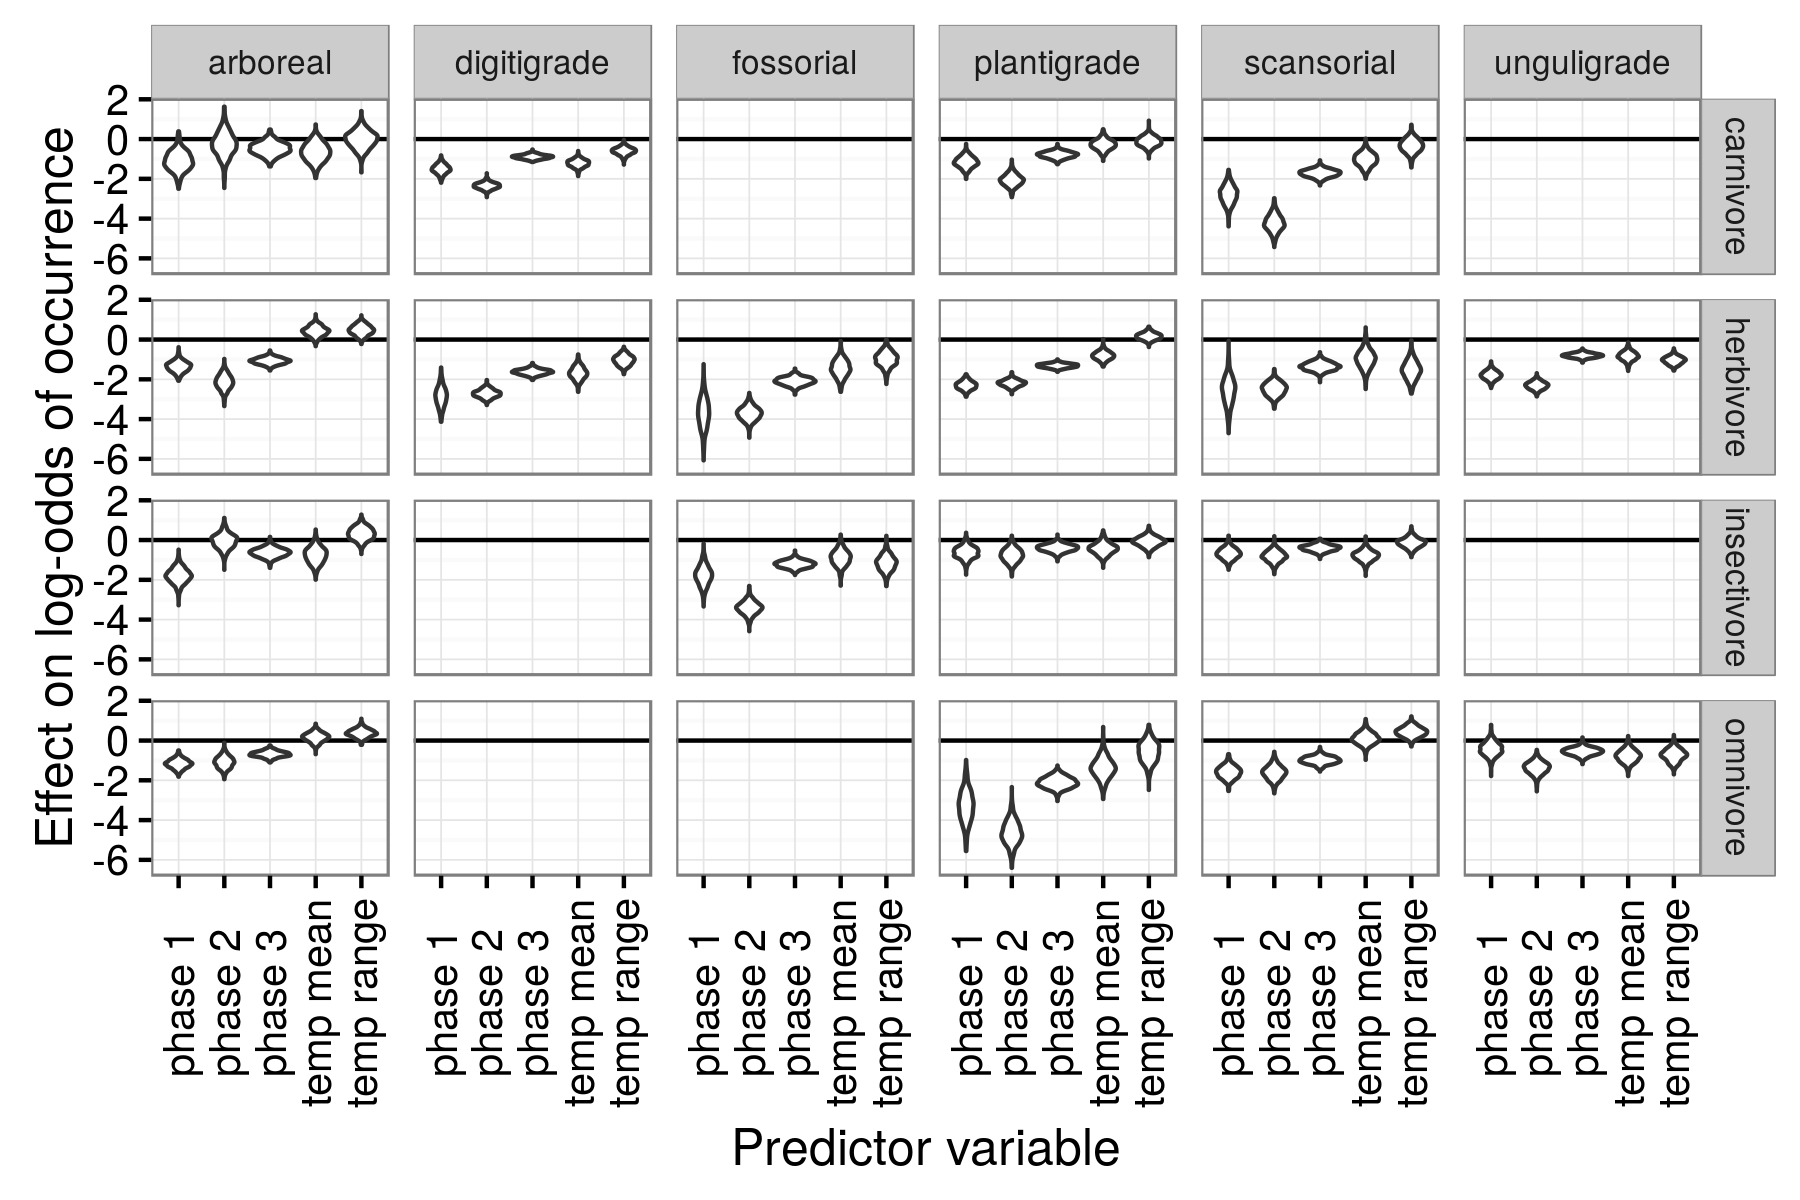
\includegraphics[width=\textwidth,height=0.8\textheight,keepaspectratio=true]{figure/group_on_ecotype}
  \caption[Effects of group-level covariates on log-odds of ecotype occurrence as estimated from the the pure-presence model]{Estimated effects of the group-level covariates describing environmental context on log-odds of species occurrence. These estimates are from the pure-presence model.} 
  \label{fig:group_pure_presence}
\end{figure}

\begin{figure}[ht]
  \centering
  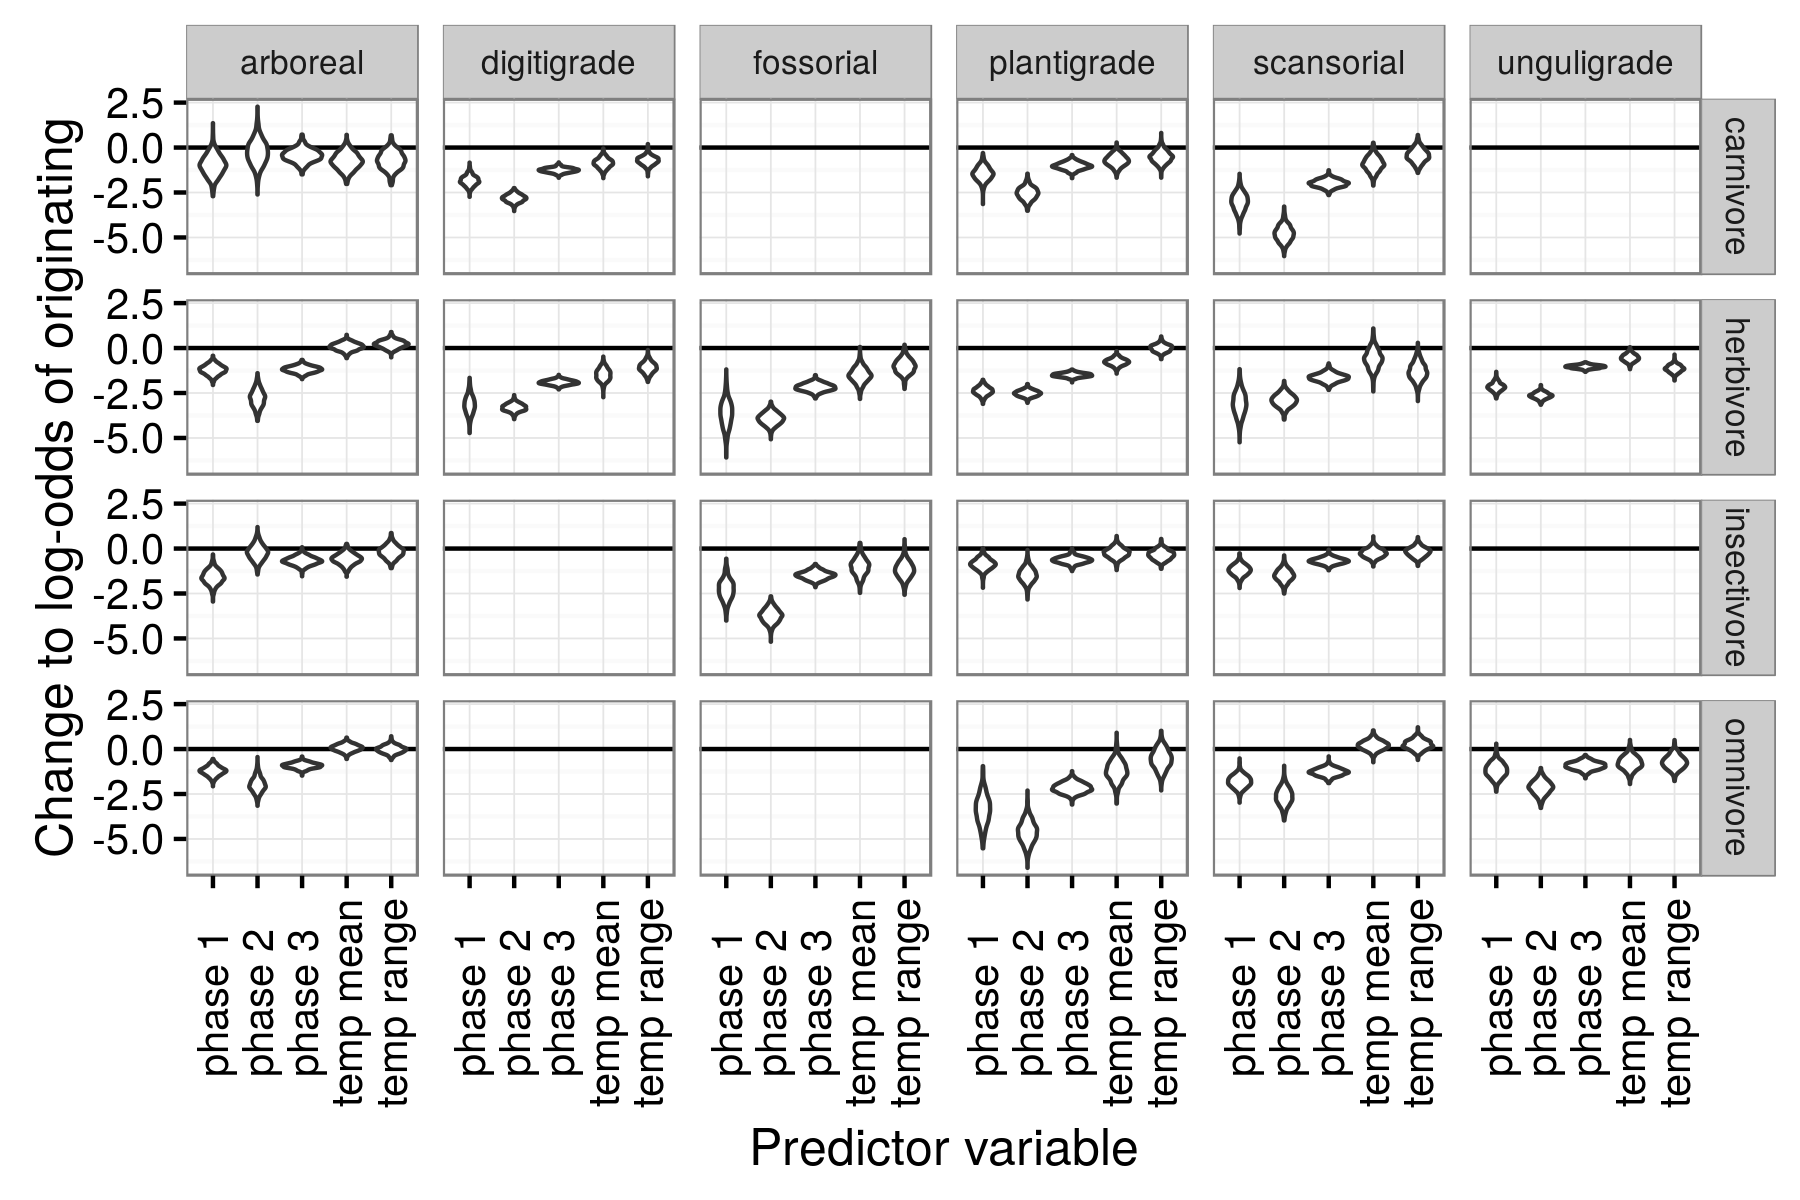
\includegraphics[width=\textwidth,height=0.8\textheight,keepaspectratio=true]{figure/group_on_origin_bd}
  \caption[Effects of group-level covariates on log-odds of ecotype origination as estimated from the the birth-death model]{Estimated effects of the group-level covariates describing environmental context on log-odds of species origination. These estimates are from the birth-death model.}
  \label{fig:group_origin_bd}
\end{figure}

\begin{figure}[ht]
  \centering
  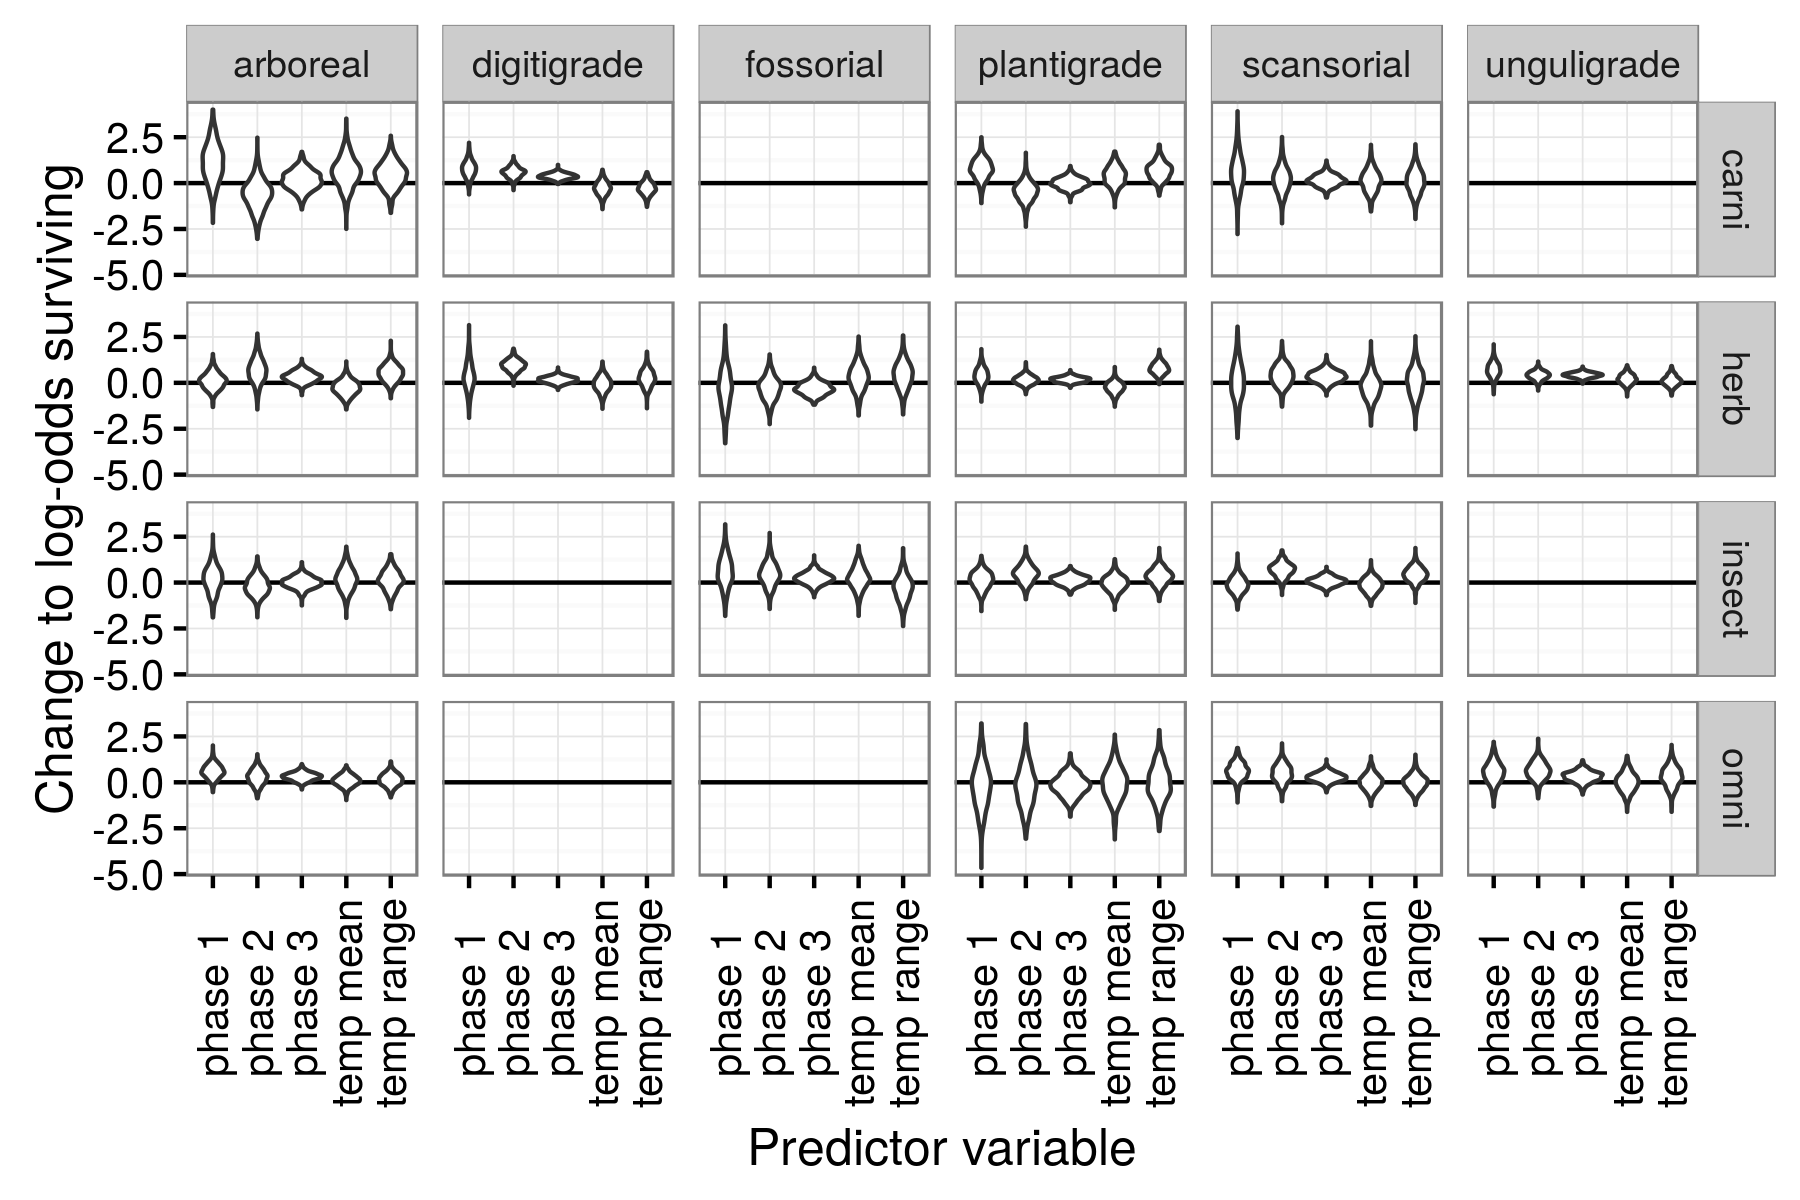
\includegraphics[width=\textwidth,height=0.8\textheight,keepaspectratio=true]{figure/group_on_survival_bd}
  \caption[Effects of group-level covariates on log-odds of ecotype survival as estimated from the the birth-death model]{Estimated effects of the group-level covariates describing environmental context on log-odds of species survlval. These estimates are from the birth-death model.}
  \label{fig:group_surv_bd}
\end{figure}





\subsection*{Analysis of diversity}


\end{document}
